%%%%%%%%%%%%%%%%%%%%%%%%%%%%%%%%%%%%%%%%%%%%%%%%%%
%%%%%%%%%%%%%%%%%%%%%%%%%%%%%%%%%%%%%%%%%%%%%%%%%%
%%
%% Based one the "beamer-greek-two" template provided 
%% by the Laboratory of Computational Mathematics, 
%% Mathematical Software and Digital Typography, 
%% Department of Mathematics, University of the Aegean
%% (http://myria.math.aegean.gr/labs/dt/)
%%
%% Adapted by John Liaperdos, October-November 2014
%% (ioannis.liaperdos@gmail.com)
%%
%% Last update: 22/06/2017 (English Support)
%%
%%%%%%%%%%%%%%%%%%%%%%%%%%%%%%%%%%%%%%%%%%%%%%%%%%
%%%%%%%%%%%%%%%%%%%%%%%%%%%%%%%%%%%%%%%%%%%%%%%%%%
%%
\PassOptionsToPackage{unicode}{hyperref}
\PassOptionsToPackage{naturalnames}{hyperref}
\documentclass{beamer} 
%\usepackage{babel}
%\usepackage[utf8]{inputenc}
\usepackage[longnamesfirst,square,numbers,comma,sort&compress]{natbib}


%%% FONT SELECTION %%%%%%%%%%%%%%%%%
%%% we choose a sans font %%%%%%%%%%
\usepackage{kmath,kerkis} 
%\usepackage[default]{gfsneohellenic} 
%%%%%%%%%%%%%%%%%%%%%%%%%%%%%%%%%%%%

\usepackage{color}
\usepackage{amsmath}
\usepackage{amssymb}
\usepackage{media9}

\usepackage{epstopdf}
\usepackage{graphicx}
\graphicspath{{./images/}}

%%
% load TEI-Pel - specific layout
\usepackage{TeiPel_En_Beamer_Layout}
\setTeipelLayout{draft,newlogo}% options: "draft", "newlogo"

%%%%%%%%%%%%%%%%%%%%%%%%%%%%%%%%%%%%%%%%%%%%%%%%%%%%%%%%%%%%
% Thesis Info %%%%%%%%%%%%%%%%%%%%%%%%%%%%%%%%%%%%%%%%%%%%%%
%%%%%%%%%%%%%%%%%%%%%%%%%%%%%%%%%%%%%%%%%%%%%%%%%%%%%%%%%%%%
	% title
		\title[This is my Title]{Comprehensive machine-learning-based analysis of microRNA-target interactions reveals variable transferability of interaction rules across species}	
	% author 
    % (In the mandatory argument "{}", separate multiple
    % authors with "\and" - use "\\" for better author name formatting
    % in the title page. In the optional argument "[]" include all
	% author names, with no "\and" or text formatting macros.)
	% Example: 
    %\author[A. Author Albert Einstein]{Anthony Author \and Albert Einstein}
		\author[A. Author]{Gilad Ben Or}
	% supervisor	
		\supervisor{Supervisor}{Isana Veksler-Lublinsky}{PhD}
	% date
		\presentationDate{October 22, 2017}
%%%%%%%%%%%%%%%%

\begin{document}

% typeset front slides
	\typesetFrontSlides

%%%%%%%%%%%%%%%%
% Your Slides Start here:

%%%%
\section{Motivaton}

%%
\subsection[Background]{MicroRNA background}
\begin{frame}{MicroRNA}
	\begin{itemize}
\item MicroRNAs (miRNAs) are small non-coding RNAs that regulate gene expression post-transcriptionally. 
\item Mature miRNAs form the core of the miRNA-induced silencing complex with Argonaute proteins (miRISC).
\item miRISC uses the sequence information in the miRNA as a guide to recognize and bind with target mRNAs.

\end{itemize}
\end{frame}

\begin{frame}{MicroRNA}
	\begin{itemize}
\item miRISC binding typically leads to translational inhibition and/or degradation of targeted mRNAs.
\item miRNAs are conserved throughout evolution and are present in the genomes of animals and plants.  
\item miRNAs have diverse functions in development and physiology and have been implicated in many human diseases.
\end{itemize}
\end{frame}

\subsection{miRNA target sites}
%%%%%%%%%%%%%%%%%%%%%%%%%%%%%%%%%%
\begin{frame}{Identification of miRNA target sites}
	\begin{itemize}
	\item The identification of miRNA target sites on mRNAs is a fundamental step in understanding miRNA involvement in cellular processes.

	\item Identifying target genes using laboratory experiments involves complex techniques.
\end{itemize}
\end{frame}

\begin{frame}{Identification of miRNA target sites}
	\begin{itemize}
\item Measuring changes in mRNA levels following miRNA over-expression or inhibition in tissue-cultured cells.
    \begin{itemize}
    \item Cons: indirect signals, exact sequences are unknown, may miss signals.
    \end{itemize}
		\pause

\item Crosslinking and immunoprecipitation (CLIP) of RNA-protein complexes that are found in direct contact.
  \begin{itemize}
    \item Cons: the identity of the specific miRNA has to be predicted bioinformatically.
    \end{itemize}

\end{itemize}
\end{frame}


\begin{frame}{Identification of miRNA target sites}
	\begin{itemize}
\item Recently, advanced methods have been developed to capture miRNAs bound to their respective targets.
\begin{itemize}
\item CLASH (Cross-linking, Ligation and Sequencing of Hybrids) \cite{helwak2013mapping}
\item CLEAR (covalent ligation of endogenous Argonaute-bound RNAs)-CLIP \cite{darnell_moore2015mirna, scheel2017global}
\item Modified iPAR-CLIP \cite{grosswendt2014unambiguous}
\end{itemize}
\item These methdos use an extra step to covalently ligate the 3' end of a miRNA and the 5' end of the associated target RNA within the miRISC. 
\end{itemize}
\end{frame}

\begin{frame}{Avaliable datasets}
% 	\begin{itemize}
% 	\item Direct experiments
% 		\begin{itemize}

% 	\item Human - 2 
% 	\item \textit{Caenorhabditis elegans (C. elegans)} - 2
% 	\item Cattle \textit{Bos taurus} -1
% 	\item Mouse - 1
% 	\end{itemize}
% 	\pause
% 		\item re-analysis of previous experiments
% 			\begin{itemize}
% \item Human - 1
% \item Mouse - 1
% 		\end{itemize}
% 	\end{itemize}

\begin{table}[h!]
\label{tbl:dataset_description}
% \begin{tabular}{ | l | l | l | l | l | }
 \resizebox{\textwidth}{!}{%
\begin{tabular}{|l|p{5cm}|p{4cm}|l|}
	\hline
	\textbf{Name} & \textbf{Cell/ Developmental stage} & \textbf{Experimental Method} & \textbf{Reference} \\
	\hline
	
% 	cattle\_MDBK & 
    ca1 &
	Madin-Darby bovine kidney (MDBK) &
	CLEAR-CLIP                        
	& \cite{scheel2017global} \\
	\hline
	
% 	celegans\_L3 & 
    ce1 &
	L3 staged & 
	Modified iPAR-CLIP & 
	\cite{grosswendt2014unambiguous}  \\
	\hline

% 	celegans\_L4 & 
    ce2 &
	Mid-L4 WT (N2)  & 
	ALG-1 iCLIP endogenous ligation & 
	\cite{broughton2016pairing} \\
	\hline

% 	human\_HEK293 & 
    h1 &
	\textbf{Human embryonic kidney293 cells (HEK293)} & 
	CLASH  & 
	\cite{helwak2013mapping} \\
	\hline
	
% 	human\_mix & 
    h2 &
	A mix of 6 datasets & 
	AGO-CLIP endogenous ligation &  
	\cite{grosswendt2014unambiguous} \\
	\hline
	
% 	human\_huh7.5 & 
    h3 &
	Human hepatoma cells (Huh-7.5) & 
	CLEAR-CLIP & 
	\cite{darnell_moore2015mirna} \\
	\hline
	
% 	mouse\_mix & 
    m1 &
	A mix of 3 datasets & 
	AGO-CLIP endogenous ligation & 
	\cite{grosswendt2014unambiguous} \\
	\hline
	
% 	mouse\_ATCC & 
    m2 &
	N2A mouse neuroblastoma (ATCC) & 
	CLEAR-CLIP & 
	\cite{darnell_moore2015mirna} \\
	\hline
\end{tabular}}
\end{table}


\end{frame}

\subsection{Research Questions}
%%%%%%%%%%%%%%%%%%%%%%%%%%%%%%%%%%

\begin{frame}{Research Questions}
	\begin{itemize}

\item We would like to study the transferability of miRNA-target interaction rules between organisms
\begin{enumerate}
% \item What are the available datasets of chimeric miRNA-target interactions from a variety of organisms?
\item What are the specifications of a standard format, to represent all the available datasets?
\item What are the high-level and raw-level features that best represent interactions?
\item What are the key features of miRNA-target interactions for each organism?
\item What is the performance of machine learning models in predicting organism interactions different from the one they have trained on?
\item What are the different factors that best explain the observed results, and do they coincide with the evolutionary distance?
\end{enumerate}

	\end{itemize}
\end{frame}


\subsection{Previous work}
%%%%%%%%%%%%%%%%%%%%%%%%%%%%%%%%%%%%%%

\begin{frame}{Previous work}

Several ML-based methods utilized chimeric miRNA-target datasets to build and evaluate models. These methods differ in several aspects:
\begin{enumerate}
\item ML approach
\item Features
\item Datasets for training and testing
\item Generation of negative data
\end{enumerate}

\end{frame}


\begin{frame}{Previous work}

\begin{table}[h!]
\centering

\caption{A summary of machine-learning based methods that utilized chimeric miRNA-target datasets in their models.}
\label{tab:toolsummary}
\centering
   \resizebox{\textwidth}{!}{%

\begin{tabular}{|l|l|l|l|l|l|}
\hline
\textbf{Tool} & \textbf{ML method} & \textbf{Datasets used for training/testing}                                     & \textbf{Independent Dataset}                                                   & \textbf{Negative interactions} & \textbf{Features} \\ \hline
chimiRic \cite{lu2016learning}      & SVM                & Human (CLASH, AGO-CLIP)                                                                                            & \begin{tabular}[c]{@{}l@{}} chimeras from \\ Mouse and \textit{C.elegans} \end{tabular}                                                              & \begin{tabular}[c]{@{}l@{}}seed matching \\ non-CLIP sites \end{tabular}                   & Small             \\ \hline
TarPmiR \cite{ding2016tarpmir}       & Random Forest      & Human (CLASH)                                                                                                         & \begin{tabular}[c]{@{}l@{}}Human (PAR-CLIP), \\ Mouse (HITS-CLIP)\end{tabular}   & \begin{tabular}[c]{@{}l@{}}Negative target sites, \\ on positive mRNAs\end{tabular}                     & 13                \\ \hline
DeepMirTar \cite{wen2018deepmirtar}   & Deep learning      & Human (CLASH) + mirRecords                                                                                            & Human (PAR-CLIP)                                                                & Mock miRNAs                          & 750               \\ \hline
miRAW \cite{pla2018miraw}        & Deep learning      & \begin{tabular}[c]{@{}l@{}}Human (intersection of: CLASH, CLIP, \\ TargetScan with Diana TarBase, mirTarBase)\end{tabular} & Human (microarray)                                                              & Experimental data                  & Raw sequence       \\ \hline
mirLSTM \cite{paker2019mirlstm}      & Deep learning      & Human (CLASH) + mirRecords                                                                                            & Experimental                                                                   & Mock miRNAs                          & Raw sequence       \\ \hline
mirTarget \cite{wang2016improving}    & SVM                & Human (CLASH, AGO-CLIP)                                                                                               & Human(microarrays)                                                              & \begin{tabular}[c]{@{}l@{}}seed matching non-CLIP sites \\ on expressed mRNAs \end{tabular}                           & 50                \\ \hline
mirTarget v4 \cite{liu2019prediction} & SVM                & \begin{tabular}[c]{@{}l@{}}Human (Intersection of \\ CLASH and microarrays) \end{tabular}                                                                                             & \begin{tabular}[c]{@{}l@{}}Mouse (HITS-CLIP), \\ Human (microarrays)\end{tabular} & \begin{tabular}[c]{@{}l@{}}seed matching non-CLIP sites \\ on expressed mRNAs \end{tabular}                          & 96                \\ \hline
\end{tabular}}
\end{table}
\end{frame}


\begin{frame}{DeepMirTar}
\begin{itemize}
\item DeepMirTar \cite{wen2018deepmirtar} is based on a stacked de-noising auto-encoder deep learning method (SdA).
\item Uses 750 different features to describe the interactions.
\item The features capture the information about the seed match, sequence composition, free energy, site accessibility, conservation, and hot-encoding of miRNAs and their target sites. 
\end{itemize}
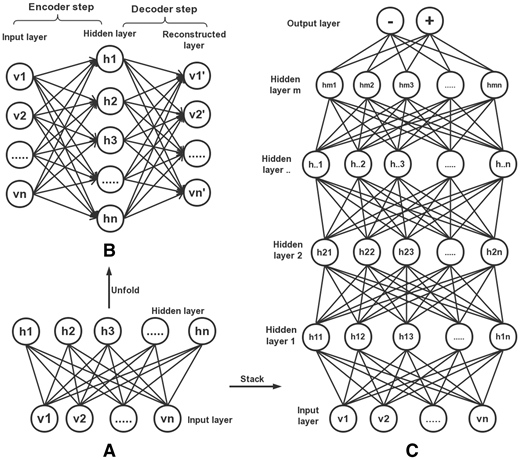
\includegraphics[width=0.5\textwidth,keepaspectratio]{images/deepmirtarsda.png}

\end{frame}

\begin{frame}{Accuracy performance}
\begin{table}[h!]
\caption{taken from deepMirTar \cite{wen2018deepmirtar}.}
\label{tab:existingmethods}
\centering
   \resizebox{\textwidth}{!}{%

\begin{tabular}{lll|l|l|}
\cline{1-2} \cline{4-5}
\multicolumn{1}{|l|}{\textbf{Methods}} & \multicolumn{1}{l|}{\textbf{ACC}} & \textbf{} & \textbf{Machine learning alg.} & \textbf{ACC}    \\ \cline{1-2} \cline{4-5} 
\multicolumn{1}{|l|}{Miranda}          & \multicolumn{1}{l|}{0.6592}       &           & DT (Decision Tree)                            & 0.8139 (0.0137) \\ \cline{1-2} \cline{4-5} 
\multicolumn{1}{|l|}{RNAhybrid}        & \multicolumn{1}{l|}{0.6988}       &           & BNB (Bernoulli Naïve Bayes)                            & 0.7570 (0.0098) \\ \cline{1-2} \cline{4-5} 
\multicolumn{1}{|l|}{PITA}             & \multicolumn{1}{l|}{0.4981}       &           & LR (Logistic Regression)                            & 0.8491 (0.0117) \\ \cline{1-2} \cline{4-5} 
\multicolumn{1}{|l|}{TargetScan v7.0a} & \multicolumn{1}{l|}{0.5801}       &           & RF (Random Forest)                             & 0.8811 (0.0090) \\ \cline{1-2} \cline{4-5} 
\multicolumn{1}{|l|}{TarPmiR}          & \multicolumn{1}{l|}{0.7446}       &           & MLP (Multi-Layer Perceptron)                            & 0.8990 (0.0099) \\ \cline{1-2} \cline{4-5} 
\multicolumn{1}{|l|}{\textbf{DeepMirTar (SdA)}} & \multicolumn{1}{l|}{0.9348}       &           & CNN-1D (Convolutional Neural Network)                         & 0.8886 (0.0145) \\ \cline{1-2} \cline{4-5} 
                                       &                                   &           & CNN-2D (Convolutional Neural Network)                         & 0.8765 (0.0169) \\ \cline{4-5} 
\end{tabular}}
\end{table}
\end{frame}

\section{Results}
%%%%%%%%%%%%%%%%%%%%%%%%%%%%%%%%%%%%%%%%%%%%%%%%%%%%%%%%
\subsection{Processing pipeline}
\begin{frame}{Processing pipeline}
\begin{itemize}
\item Transform and unify the datasets' different data formats.
\begin{enumerate}
\item Retrieve missing miRNA sequences (miRBase).
\item Extract target sequences based on the genomic coordinates. 
\item Blast \cite{altschul1990basic_blast} to match the target mRNA sequences against the 3'UTRs (Ensembl Biomart).
\item Duplex generation using ViennaRNA suite (RNAduplex) \cite{lorenz2011viennarna}.
\item Keeping canonical and non-canonical seed interactions only.
\end{enumerate}
\item Enable, with a relatively low effort, to add more data sources to the analysis.
\end{itemize}
 \end{frame}



\begin{table}[h!]
\caption{Data processing pipeline}
\label{tab:preprocess}
 \resizebox{\textwidth}{!}{%
\begin{tabular}{|l|c|c|c|c|c|}
\hline
\textbf{Paper}       & \cite{helwak2013mapping} & \cite{grosswendt2014unambiguous} & \cite{scheel2017global} & 
\cite{broughton2016pairing} & \cite{darnell_moore2015mirna} \\ \hline
\textbf{Datasets}  & h1 & ce1, h2, m1 & ca1                & ce2      & h3, m2  \\ \hline
\textbf{miRNA sequence}  & \checkmark  & \checkmark           &  mirbase & mirbase  & mirbase \\ \hline
\textbf{Target sequence} & \checkmark  & \checkmark           & \checkmark                  & wormbase & UCSC genome browser  \\ \hline
\textbf{Site region}      & \multicolumn{5}{c|}{Ensembl Biomart + Blast}                                 \\ \hline
\textbf{Duplex structure}     & \multicolumn{5}{c|}{Vienna RNAduplex}                                \\ \hline
\textbf{Seed Filter} & \multicolumn{5}{c|}{Canonical and non-canonical seeds only}                \\ \hline
\end{tabular}}

\end{table}



\begin{frame}{Summary of the data processing pipeline}

\begin{table}[h!]
      \label{tal:pipeline_summary}
                 \begin{threeparttable}
                    \resizebox{\textwidth}{!}{%
 \resizebox{\textwidth}{!}{%

      \begin{tabular}{|l|l|l|l|l|l|l|l|l|}

\hline
\textbf{Dataset}                                                                                   & \textbf{ca1}     & \textbf{ce1}   & \textbf{ce2}   & \textbf{h1}     & \textbf{h2}     & \textbf{h3}     & \textbf{m1}    & \textbf{m2}      \\ \hline
No. of interactions                                                                      & 296,297 & 3,627 & 4,920 & 18,514 & 10,567 & 32,712 & 1,986 & 130,094 \\ \hline
No. of interactions in 3'UTRs                                                                 & 30,534  & 1,704 & 1,206 & 8,507  & 2,039  & 4,634  & 902   & 33,100  \\ \hline
\textbf{\begin{tabular}[c]{@{}l@{}}Final dataset\\ (canonical \& non-canonical\\ interactions)\end{tabular}} & \textbf{18,204} & \textbf{1,176} & \textbf{992} & \textbf{5,137} & \textbf{1,150} & \textbf{2,846} & \textbf{537} & \textbf{17,574} \\ \hline
\end{tabular} }}
\
     \end{threeparttable}
\end{table}
\end{frame}

\section{Datasets' characteristics}
%%%%%%%%%%%%%%%%%%%%%%%%%%%%%%%%%%%%%%%%%%

\begin{frame}{Summary of the data processing pipeline}

\begin{figure}[h!]
  \caption{\textbf{Cumulative sum of miRNA sequence appearances in the examined datasets}}
      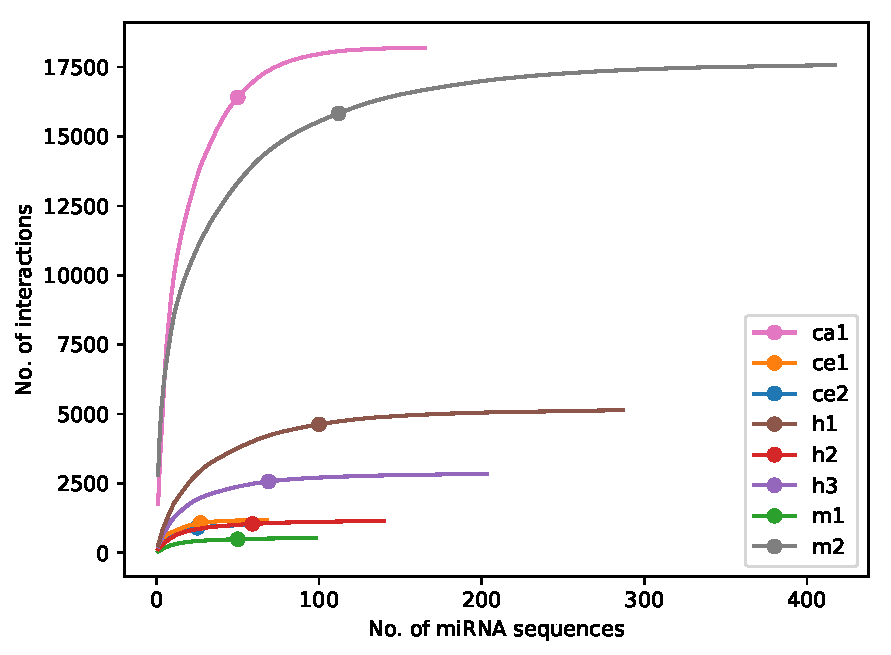
\includegraphics[width=\textwidth]{images/1_mirna_dist.pdf}
      \label{fig:datasetplot}
      \caption*{Each curve corresponds to the cumulative sum of one of the datasets, where the bold points indicate the minimum number of unique miRNA sequences needed to represent 90\% of the interactions within a dataset. The height of a curve represents the size of the dataset, and the width of a curve represents the number of unique miRNA sequences that comprise the dataset.}
      \end{figure}
\end{frame}

\begin{frame}{Summary of the data processing pipeline}

\begin{figure}[h!]
  \caption{\textbf{Classification of the miRNA-target duplexes based on their base-pairing patterns}} 
    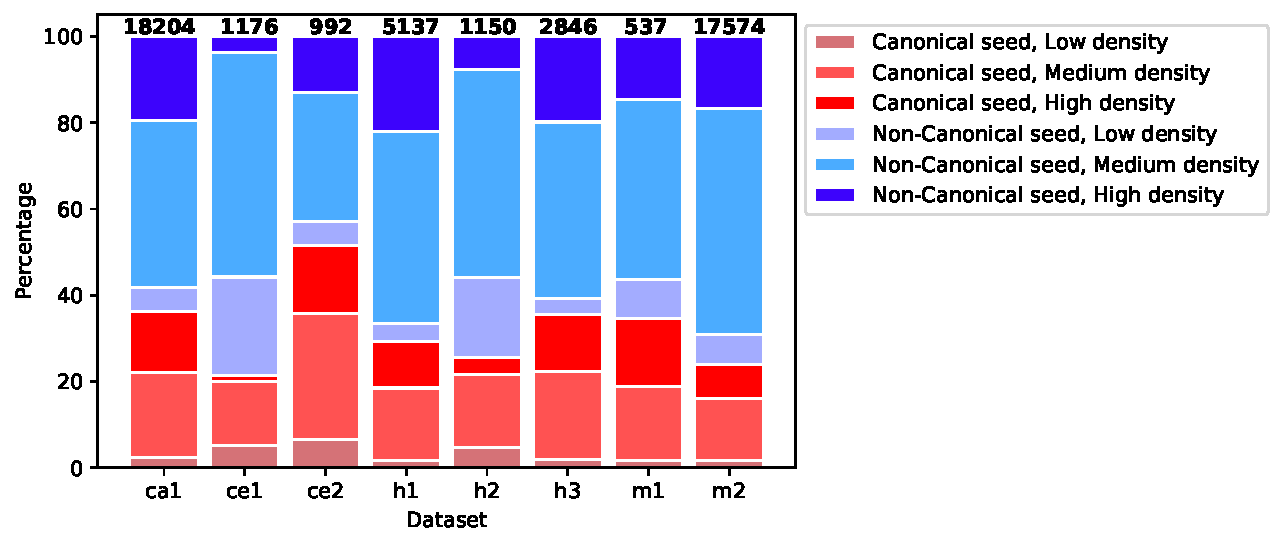
\includegraphics[width = 1\textwidth]{images/2_seed_type_positive2.pdf}
      \label{fig:seed_type_pos}
      \caption*{Distribution of miRNA-target duplexes across 6 classes according to the seed type (canonical and non-canonical) and to the base-pairing density (low: less than 11bp, medium: 11-16bp and high: more than 16bp).}

      \end{figure}
\end{frame}
      




% \begin{frame}{Slide Title \#4}
% 	\begin{example}
% 		<1->First example. 
% 	\end{example}
% 	\begin{example}
% 		<2->Second example.
% 	\end{example}
% \end{frame}



% \begin{frame}{Slide Title \#1}
% 	\framesubtitle{Slide subtitle \#1}
% 	\begin{itemize}
% 		\item Use the \texttt{itemize} environment frequently.
% 		\pause
% 		\item Use short sentences and phrases.
% 		\pause
% 		\item In this presentation we use the \textbackslash{}\texttt{pause} macro.
% 	\end{itemize}
% \end{frame}

% \begin{frame}{Slide Title \#2}
% 	\begin{itemize}
% 		\item <1->You can define the order of appearance.
% 		\item <3->Like here.
% 		\item <2->This is the second item to appear.
% 	\end{itemize}
% \end{frame}

% \begin{frame}{Slide Title \#3}
% 	\begin{block}
% 		<1->{}
% 		\begin{itemize}
% 			\item Group without title.
% 			\item Appears for all slides.
% 		\end{itemize}
% 	\end{block}
% 	\begin{exampleblock}
% 		<2->{Group title}
% 		\begin{itemize}
% 			\item $e^{i\pi}=-1$.
% 			\item $e^{i\pi/2}=i$.
% 		\end{itemize}
% 	\end{exampleblock}
% \end{frame}

% %%
% \subsection{Previous work}

% \begin{frame}{Slide Title \#4}
% 	\begin{example}
% 		<1->First example. 
% 	\end{example}
% 	\begin{example}
% 		<2->Second example.
% 	\end{example}
% \end{frame}

% \begin{frame}{Slide Title \#5}
% 	\begin{center}
% 		Table example \\[12pt]
% 		\begin{tabular}{c||c|c|c|}
% 			& \textbf{col 1} & \textbf{col  2} & \textbf{col 3} \\
% 			\hline
% 			\hline
% 			\textbf{row 1} & 11 & 12 & 13 \\
% 			\hline
% 			\textbf{row 2} & 21 & 22 & 23 \\
% 		\end{tabular}
%     \end{center}
% \end{frame}

% \begin{frame}{Slide Title \#6}
% 	\begin{center}
% 		Figure example \\[12pt]
% 		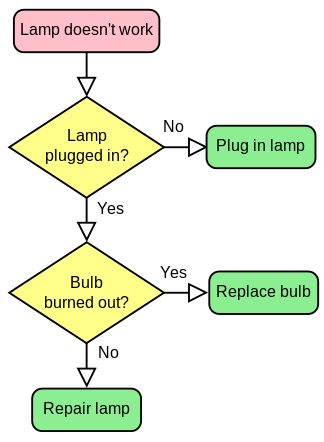
\includegraphics[width=0.35\textwidth,keepaspectratio]{LampFlowchart.png}
% 		\\
% 		\footnotesize(source: \textlatin{Wikipedia})
%     \end{center}
% \end{frame}

% \begin{frame}{Slide Title \#7}
% 	\centering
% 	Math examples \\[12pt]
% 	\begin{equation}
%         	B'=-\nabla \times E
% 	\end{equation}
% 	\begin{equation*}
%         	E'=\nabla \times B - 4\pi j
% 	\end{equation*}
% \end{frame}

% %%%%
% \section{Results / contribution}

% %%
% \subsection{Main results}

% \begin{frame}{Summary}
%   	\begin{alertblock}{Attention}
%   		\textlatin{This is an important alert}
%   	\end{alertblock}
% \end{frame}

% %
% \subsection{Subsection title}

% \begin{frame}{Summary}
% 	\begin{itemize}
% 		\item The \textcolor{red}{first main message} of our talk.
% 		\item The \textcolor{red}{second main message} of our talk.
% 		\item Maybe a \textcolor{red}{third message}, but ... no more.
% 	\end{itemize}
% 	\vskip0pt plus.5fill
% 	\begin{itemize}
% 		\item Conclusion.
% 	\end{itemize}
% 	\begin{itemize}
% 		\item Future work.
% 		\item Discussion.
% 	\end{itemize}
% \end{frame}

\begin{frame}{References}
	\begin{thebibliography}{2}
\bibliographystyle{abbrv}  
\bibliography{thesis}
% 		\beamertemplatebookbibitems
% 		\bibitem{Author1990}A.\ Author. \newblock\emph{Handbook of Everything}.\newblock
% \textlatin{Some Press, \oldstylenums{1990}}.

% 		\beamertemplatearticlebibitems
% 		\bibitem{Someone2002}B.\ Author.\newblock On this and that\emph{.}
% \newblock\emph{Journal on This and That}. 
% \oldstylenums{2}(\oldstylenums{1}):\oldstylenums{50}--\oldstylenums{100}, 
% \oldstylenums{2000}.
	\end{thebibliography}
\end{frame}

%%
\end{document}